\section{Device/Service Discovery}\label{sec:discovery}
Device discovery is one outstanding benefit when we deploy IoT system on ICN network.In the traditional IP-based IoT system, in order to use human-readable or application-readable name to identify sensing and actuating device, middleware usually handle name to IP/PORT address mapping, with the IP transport oblivous of application delivery. And the middleware can be complex and require amount of development time. IoT entities have been typically identified using manufacturer assigned IDs, which can be cryptographic ID, human readable name etc.These names are mapped to its locator-ID and used as de-facto IDs in the Internet today, that has issues with dynamic properties such as mobility. In contrast, ICN can use these natives IDs without any further mapping, and scale control and forwarding overhead through active participation by the network. Middleware somehow will be less significant as it is in IP network.  
%Look for jeff's paper here

In NDN lighting system\cite{},it assumes that lighting device comes with a manufacture assigned public key, a shared secret for initialized authorization, and a well-known NDN name, such as /ndn/lighting for discovery. First, a new device register itself and publish its public key.The configuration manager(CM) will periodically express its interest using a well-known service name, such as ndn/lighting. If a node connect to a new device, it reply a corresponding data packet with new device information. Lastly, the CM assigns a application-specific name, authenticates fixture by a shared secret.    

\subsection{Device/Service Discovery in Mobilityfirst}\label{sec:discoverymf}
In MobilityFirst IoT architecture, we embrace locator/ID split technique for device mobility.Also, device/service separation design is introduced here to support current low power device in a homogeneous network environment.We assumes that all IoT devices only carry a manufacturer serial number, which could be used to derive a GUID from Name Certificate and Resolution Service(NCRS)\cite{}.The IoT end device access point(EDAP), i.e. sink,fixture or even mobile phone for wearable sensor, utilize GUID to identify their service type, such as environment sensing,light control or health sensing.Once a new device attaches to a sink or fixture, it will announce its serial number as GUID, EDAP performs a GNRS insert with entry of Device GUID -> Service GUID mapping. A configuration service(CS) running on the remote server query GNRS server with Service GUID periodically. If the new device has been inserted by EDAP, query result will contain certain GUIDs.
\begin{figure}
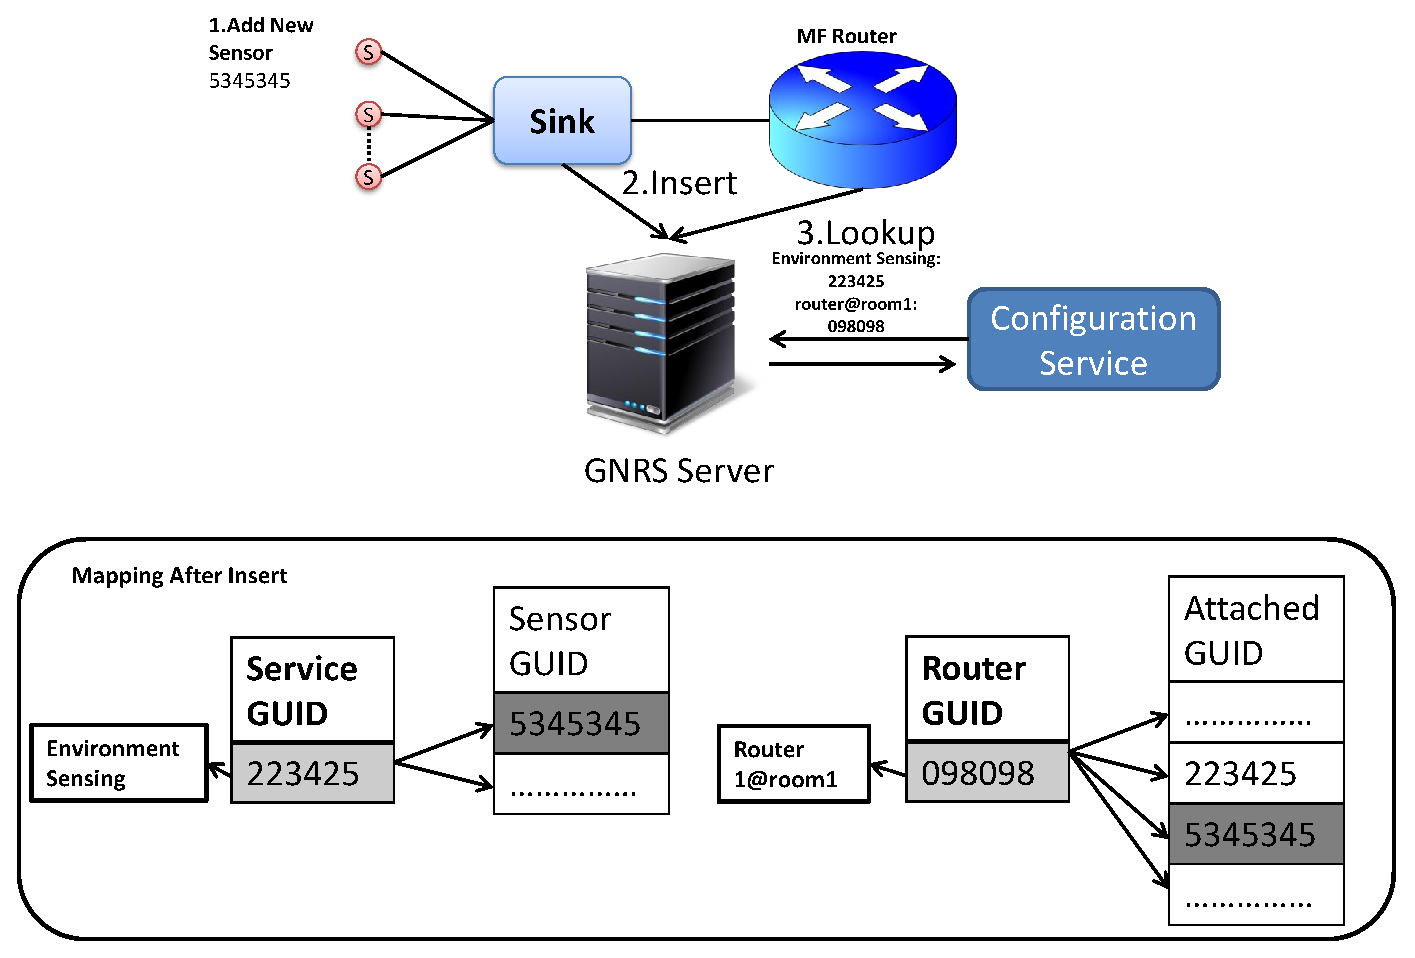
\includegraphics[width=3.00in,height=2.00in]{discovery.eps}
\caption{Three Steps for Discovery}
\label{fig:disc}
\end{figure}
Shown as Figure ~\ref{fig:disc}, a new wireless sensor dispose in a room, express itself with serial number 12345 to the nearest EDAP. EDAP is powered and relative consistent, so that we can pre-configure the service type for the it, i.e. assign a GUID or use its serial number to represent the service type. Once EDAP receive the message from the new sensor, it first looks up the local stack to confirm it has not been added before. Sensor GUID(12345) -> Service GUID(67890) mapping is inserted to GNRS server, if it does not exist in local stack. Configuration Service periodically looks up for  Service GUID(67890), and the new GUID(12345) will be  in the result list if it has been inserted. In our example, since the low power sensor has limited bandwidth and store cache, its GUID can be consistent and require no dual-way authentication. After checking the local database, CS register the new device to the IoT server if it has not being stored, in which resource and subscription membership being managed.
%do we need to include the authentication process for other device?

          

%For example, a new temperature wireless sensor comes with a serial number 1234, attaches to a EDAP, i.e. a sink node. The GUID of the sink node represents a certain service type  temperature sensing